\chapter{Disentanglement and $\beta$-VAEs}
\label{ch:beta_vae}

\section{The Quest for Factored Representations}

A central aspiration of unsupervised learning is to discover representations that carve nature at its joints. In the physical world, sensory observations are generated by the complex interaction of independent generative factors. When we look at a scene, the pixel intensities on our retina are the entangled result of lighting conditions, object geometry, color, and viewpoint. To human perception, however, these factors are distinct and independently manipulable. We can imagine the same object painted a different color, or viewed from a different angle, without altering its fundamental identity.

In the parlance of deep learning, representations that successfully separate these independent sources of variation are said to be \textit{disentangled}. A perfectly disentangled latent space aligns its coordinate axes with the true, underlying generative factors of the data. If the representation is an $M$-dimensional vector $z$, a change in a single dimension $z_i$ should correspond to a change in exactly one ground-truth factor (e.g., the azimuth angle of a face), while leaving all other factors invariant.

The Auto-Encoding Variational Bayes framework, developed in Chapters 12 and 13, provides a powerful generative mechanism but does not inherently guarantee disentanglement. The standard Variational Autoencoder (VAE) optimizes the Evidence Lower Bound (ELBO), which balances the reconstruction fidelity of the data against the divergence of the approximate posterior $q_\phi(z|x)$ from a prior $p(z)$. While this forces the latent space to be continuous and well-behaved, the standard VAE often learns entangled representations where a single semantic concept is distributed across multiple latent dimensions.

The $\beta$-VAE, introduced by Higgins et al., elegantly tackles this limitation through a minimal modification to the standard ELBO. By introducing an adjustable hyperparameter $\beta > 1$, the $\beta$-VAE places a heavier penalty on the Kullback-Leibler (KL) divergence between the approximate posterior and the prior. 

Why should penalizing the KL divergence induce disentanglement? The standard prior $p(z)$ is typically chosen to be an isotropic multivariate Gaussian, $p(z) = \mathcal{N}(0, I)$. A crucial property of this prior is that its components are statistically independent: $p(z) = \prod_{j} p(z_j)$. By forcing the aggregate posterior to closely match this factorized prior, the $\beta$-VAE objective applies immense pressure on the latent dimensions to become independent of one another. Assuming the true data-generating process relies on independent factors, matching the independent structure of the prior encourages the model to align its latent dimensions with these true factors, spontaneously yielding disentanglement.

This intuitive mechanism, however, masks a deeper information-theoretic phenomenon. When we heavily penalize the KL divergence to the prior, we are simultaneously restricting the information capacity of the latent bottleneck. The network is forced to discard the complex, high-order correlations that entangle variables, retaining only the most statistically independent and prominent features. In this chapter, we will strip away the heuristic explanations and rigorously analyze the $\beta$-VAE objective. We will decompose the KL divergence penalty to reveal the exact terms responsible for disentanglement, mathematically connect it to the Information Bottleneck principle, and demonstrate the unavoidable theoretical limits of purely unsupervised disentangled representation learning.

\section{The Information-Theoretic Foundations of $\beta$-VAE}

We begin by formally defining the $\beta$-VAE objective. Let $x \in \mathcal{X}$ be the observed data and $z$ be the continuous latent variables. The encoder (inference model) is parameterized by $\phi$ as $q_\phi(z|x)$, and the decoder (generative model) is parameterized by $\theta$ as $p_\theta(x|z)$.

\begin{definition}[$\beta$-VAE Objective]
For a given data point $x \sim P_{\text{data}}$, the $\beta$-VAE minimizes the following negative log-likelihood bound:
\begin{equation}
    \mathcal{L}_\beta(\theta, \phi; x) = -\mathbb{E}_{q_\phi(z|x)}[\log p_\theta(x|z)] + \beta D_{\text{KL}}(q_\phi(z|x) \parallel p(z))
\end{equation}
where $\beta \geq 0$ is the regularization coefficient. The standard VAE is recovered when $\beta = 1$.
\end{definition}

This modification can be derived rigorously from a constrained optimization perspective using the Information Bottleneck (IB) principle (Chapter 8). Suppose we wish to maximize the reconstruction likelihood, but we are subject to a strict upper bound on the channel capacity between the input $X$ and the latent space $Z$.

\begin{theorem}[Mutual Information Bound on the Latent Space]
\label{thm:mi_bound}
The expected KL divergence between the approximate posterior $q_\phi(z|x)$ and the prior $p(z)$ is a strict upper bound on the mutual information $I(X; Z)$ between the data and the latent representation under the empirical data distribution $p_{\text{data}}(x)$. Specifically,
\begin{equation}
    \mathbb{E}_{p_{\text{data}}(x)} \left[ D_{\text{KL}}(q_\phi(z|x) \parallel p(z)) \right] = I(X; Z) + D_{\text{KL}}(q(z) \parallel p(z))
\end{equation}
where $q(z) = \mathbb{E}_{p_{\text{data}}(x)}[q_\phi(z|x)]$ is the aggregate posterior.
\end{theorem}

\begin{proof}
Let us write the expected KL divergence explicitly:
\begin{align}
    \mathbb{E}_{p_{\text{data}}(x)} \left[ D_{\text{KL}}(q_\phi(z|x) \parallel p(z)) \right] &= \int p_{\text{data}}(x) \int q_\phi(z|x) \log \frac{q_\phi(z|x)}{p(z)} dz dx \\
    &= \iint p_{\text{data}}(x) q_\phi(z|x) \left( \log \frac{q_\phi(z|x)}{q(z)} + \log \frac{q(z)}{p(z)} \right) dz dx \\
    &= \iint p_{\text{data}}(x) q_\phi(z|x) \log \frac{q_\phi(z|x)}{q(z)} dz dx + \int \left( \int p_{\text{data}}(x) q_\phi(z|x) dx \right) \log \frac{q(z)}{p(z)} dz \\
    &= I(X; Z) + \int q(z) \log \frac{q(z)}{p(z)} dz \\
    &= I(X; Z) + D_{\text{KL}}(q(z) \parallel p(z))
\end{align}
Since the Kullback-Leibler divergence is non-negative ($D_{\text{KL}}(q(z) \parallel p(z)) \geq 0$), it follows that $\mathbb{E}_{p_{\text{data}}(x)} \left[ D_{\text{KL}}(q_\phi(z|x) \parallel p(z)) \right] \geq I(X; Z)$.
\end{proof}

\begin{figure}[htbp]
    \centering
    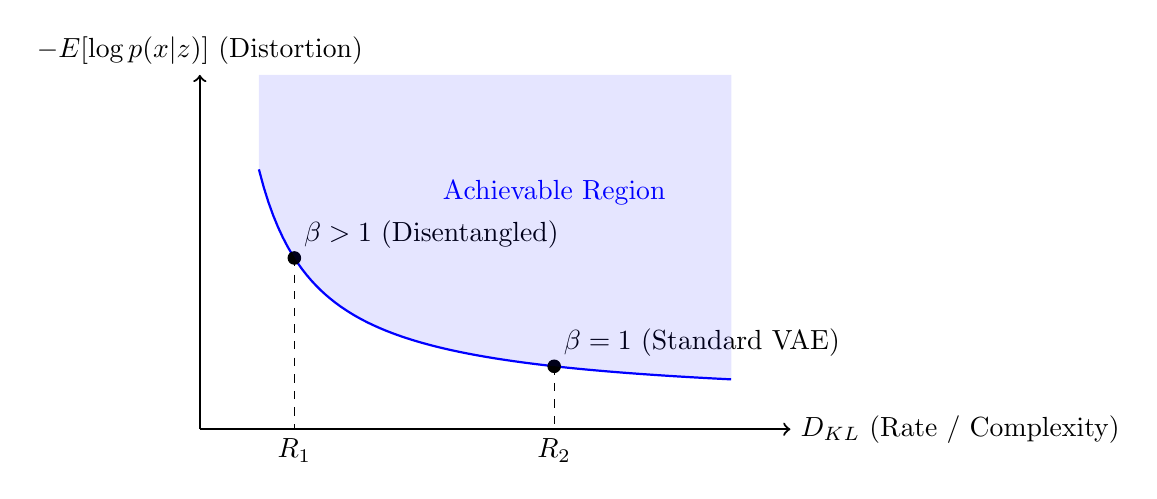
\begin{tikzpicture}[scale=1.5]
        % Axes
        \draw[->, thick] (0,0) -- (5,0) node[right] {$D_{\text{KL}}$ (Rate / Complexity)};
        \draw[->, thick] (0,0) -- (0,3) node[above] {$-\mathbb{E}[\log p(x|z)]$ (Distortion)};
        
        % Curve
        \draw[thick, blue, domain=0.5:4.5, samples=100] plot (\x, {1/\x + 0.2});
        
        % Points
        \filldraw[black] (0.8, 1.45) circle (1.5pt) node[anchor=south west] {$\beta > 1$ (Disentangled)};
        \filldraw[black] (3.0, 0.533) circle (1.5pt) node[anchor=south west] {$\beta=1$ (Standard VAE)};
        
        % Feasible region
        \fill[blue, opacity=0.1] (0.5, 3) -- plot[domain=0.5:4.5] (\x, {1/\x + 0.2}) -- (4.5, 3) -- cycle;
        \node[blue] at (3, 2) {Achievable Region};
        
        % Labels for Rate
        \draw[dashed] (0.8, 1.45) -- (0.8, 0) node[below] {$R_1$};
        \draw[dashed] (3.0, 0.533) -- (3.0, 0) node[below] {$R_2$};
    \end{tikzpicture}
    \caption{The Information Bottleneck interpretation of the $\beta$-VAE. By increasing $\beta$, we force the model to operate at a lower rate ($R_1 < R_2$), increasing the bottleneck pressure. This reduction in capacity forces the network to abandon entangled representations in favor of the most statistically independent, fundamental factors.}
    \label{fig:beta_vae_tradeoff}
\end{figure}

This theorem provides profound insight into the $\beta$-VAE. The objective is mathematically equivalent to minimizing the distortion (reconstruction error) subject to a Lagrangian penalty on the information channel capacity between data and latents. When $\beta > 1$, we aggressively throttle this capacity.

\section{Decomposition of the Evidence Lower Bound}

To understand precisely how disentanglement emerges, we must analyze the structure of the aggregate posterior $q(z)$. Assuming the latent space is $D$-dimensional, $z = [z_1, z_2, \dots, z_D]^\top$, the factorized prior is $p(z) = \prod_{j=1}^D p(z_j)$.

\begin{theorem}[KL Decomposition]
\label{thm:kl_decomp}
The expected KL divergence penalty in the $\beta$-VAE objective decomposes into three distinct information-theoretic terms:
\begin{equation}
    \mathbb{E}_{p_{\text{data}}(x)} \left[ D_{\text{KL}}(q_\phi(z|x) \parallel p(z)) \right] = I(X; Z) + TC(Z) + \sum_{j=1}^D D_{\text{KL}}(q(z_j) \parallel p(z_j))
\end{equation}
where $q(z_j)$ is the marginal distribution of the $j$-th latent dimension, and $TC(Z)$ is the Total Correlation of the latent variables.
\end{theorem}

\begin{proof}
By Theorem \ref{thm:mi_bound}, we know the expected KL is equal to $I(X;Z) + D_{\text{KL}}(q(z) \parallel p(z))$. We now decompose the second term, the marginal KL divergence to the prior:
\begin{align}
    D_{\text{KL}}(q(z) \parallel p(z)) &= \int q(z) \log \frac{q(z)}{p(z)} dz \\
    &= \int q(z) \log \frac{q(z)}{\prod_{j=1}^D q(z_j)} \frac{\prod_{j=1}^D q(z_j)}{\prod_{j=1}^D p(z_j)} dz \\
    &= \int q(z) \log \frac{q(z)}{\prod_{j=1}^D q(z_j)} dz + \int q(z) \sum_{j=1}^D \log \frac{q(z_j)}{p(z_j)} dz \\
    &= D_{\text{KL}}\left( q(z) \parallel \prod_{j=1}^D q(z_j) \right) + \sum_{j=1}^D \int q(z_j) \log \frac{q(z_j)}{p(z_j)} dz_j \\
    &= TC(Z) + \sum_{j=1}^D D_{\text{KL}}(q(z_j) \parallel p(z_j))
\end{align}
Substituting this back into the identity from Theorem \ref{thm:mi_bound} completes the proof.
\end{proof}

\begin{figure}[htbp]
    \centering
    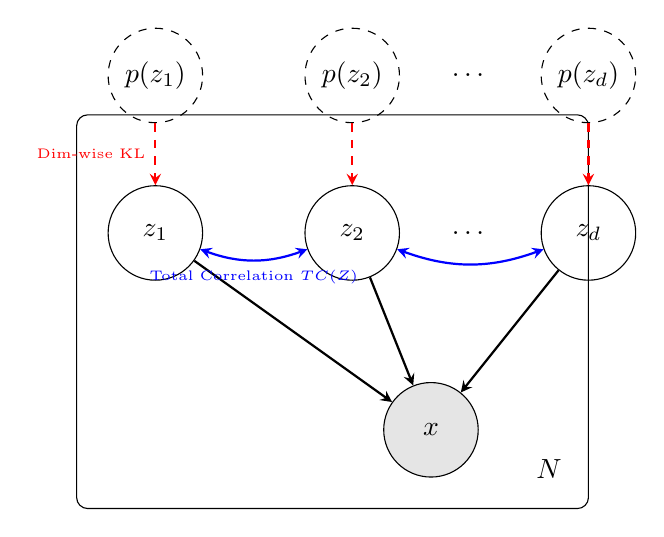
\begin{tikzpicture}[
        node distance=2.5cm,
        obs/.style={circle, draw, fill=gray!20, minimum size=1.2cm},
        lat/.style={circle, draw, minimum size=1.2cm},
        edge/.style={->, >=stealth, thick}
    ]
        % Prior nodes
        \node[lat, dashed] (pz1) {$p(z_1)$};
        \node[lat, dashed, right of=pz1] (pz2) {$p(z_2)$};
        \node[right of=pz2, node distance=1.5cm] (dots1) {\dots};
        \node[lat, dashed, right of=dots1, node distance=1.5cm] (pzd) {$p(z_d)$};
        
        % Latent nodes
        \node[lat, below of=pz1, node distance=2cm] (z1) {$z_1$};
        \node[lat, below of=pz2, node distance=2cm] (z2) {$z_2$};
        \node[below of=dots1, node distance=2cm] (dots2) {\dots};
        \node[lat, below of=pzd, node distance=2cm] (zd) {$z_d$};
        
        % Observation node
        \node[obs, below of=z2, node distance=2.5cm, xshift=1cm] (x) {$x$};
        
        % Plate
        \draw[rounded corners] (-1, -5.5) rectangle (5.5, -0.5);
        \node at (5, -5) {$N$};
        
        % Edges
        \draw[edge] (z1) -- (x);
        \draw[edge] (z2) -- (x);
        \draw[edge] (zd) -- (x);
        
        \draw[edge, dashed, red] (pz1) -- (z1) node[midway, left] {\tiny Dim-wise KL};
        \draw[edge, dashed, red] (pz2) -- (z2);
        \draw[edge, dashed, red] (pzd) -- (zd);
        
        \draw[<->, >=stealth, thick, blue] (z1) to[bend right=20] node[midway, below] {\tiny Total Correlation $TC(Z)$} (z2);
        \draw[<->, >=stealth, thick, blue] (z2) to[bend right=20] (zd);
        
    \end{tikzpicture}
    \caption{The decomposition of the $\beta$-VAE penalty. The objective implicitly penalizes the dimension-wise KL divergence (red, forcing marginals to match the prior), the Total Correlation (blue, forcing latent variables to be independent), and the mutual information $I(X;Z)$ (the dependence between $x$ and $z$).}
    \label{fig:beta_vae_decomp}
\end{figure}

Let us analyze the three resultant penalty terms:
\begin{enumerate}
    \item \textbf{Index-Code Mutual Information, $I(X; Z)$:} Penalizing this term explicitly restricts the channel capacity, acting as an Information Bottleneck. It forces the representation to be highly compressed.
    \item \textbf{Total Correlation, $TC(Z)$:} This is a generalization of mutual information to multiple variables. It equals zero if and only if the latent variables $z_j$ are perfectly independent under the aggregate posterior $q(z)$. \textit{This is the core mechanism that drives disentanglement.} By multiplying the expected KL by $\beta > 1$, we place an immense penalty on $TC(Z)$, forcing the network to discover statistically independent latent representations.
    \item \textbf{Dimension-wise KL, $\sum_j D_{\text{KL}}(q(z_j) \parallel p(z_j))$:} This acts as a regularizer to ensure the marginal distribution of each latent dimension does not collapse or diverge infinitely far from the standard normal prior.
\end{enumerate}

\section{Numerical Example: Phase Transitions in Linear $\beta$-VAE}

To concretize this, consider a linear $\beta$-VAE. Suppose the true data is generated as $x \sim \mathcal{N}(0, \Sigma_x)$ where $x \in \mathbb{R}^N$. The generative model is $p_\theta(x|z) = \mathcal{N}(Wz, \sigma^2 I)$ and the prior is $p(z) = \mathcal{N}(0, I)$ for $z \in \mathbb{R}^K$. The approximate posterior is $q_\phi(z|x) = \mathcal{N}(Vx, \text{diag}(\sigma_{z}^2))$.

If we optimize the $\beta$-VAE objective analytically, we observe a phenomenon known as \textit{posterior collapse}, heavily dependent on the value of $\beta$. Let $\lambda_k$ be the $k$-th eigenvalue of the data covariance matrix $\Sigma_x$, ordered such that $\lambda_1 \geq \lambda_2 \geq \dots \geq \lambda_K$.

For a given dimension $k$ in the latent space, if $\beta$ is sufficiently large, specifically if:
\begin{equation}
    \beta > \frac{\lambda_k}{\sigma^2}
\end{equation}
then the optimal solution dictates that the $k$-th latent dimension completely collapses to the prior: $V_k = 0$ (where $V_k$ is the $k$-th row of $V$) and $\sigma_{z,k}^2 = 1$. The network entirely severs the mutual information between $x$ and $z_k$. 

As $\beta$ decreases, dimensions "activate" sequentially, starting with the one aligned with the largest principal component $\lambda_1$. This demonstrates how $\beta$ acts as a strict information throttle: it prunes away latent dimensions that capture low-variance (and thus, less informative) factors of variation, forcing the model to allocate its limited channel capacity exclusively to the most dominant, independent factors of the data.

\begin{horizon}
It is mathematically proved that purely unsupervised learning of disentangled representations is fundamentally impossible without structural inductive biases. Locatello et al. (2019) elegantly demonstrated that for any perfectly disentangled generative model, there exists an infinite family of alternative, highly entangled models that produce the exact same marginal data distribution $p(x)$. Because the ELBO depends on the data only through the marginal likelihood, the $\beta$-VAE—and any purely unsupervised method—cannot theoretically distinguish between the true disentangled model and an entangled equivalent.

It is conjectured that the empirical success of $\beta$-VAEs on specific datasets is driven not purely by the objective function, but by the implicit regularization provided by neural network architectures (such as the locality of convolutions) and the specific hyperparameters chosen. Future work might show that weak supervision, temporal continuity in sequential data, or carefully engineered non-Gaussian priors are theoretically necessary conditions to guarantee the identifiability of true latent factors. An open question remains whether we can design foundational models that inherently leverage these multi-view or temporal symmetries to bypass these impossibility theorems, shifting the field from heuristic regularization to guaranteed disentanglement.
\end{horizon}

\section{Summary}
\begin{itemize}
    \item Disentanglement seeks representations where single latent units correspond to single, independent factors of variation in the generative process of the data.
    \item The $\beta$-VAE objective introduces a hyperparameter $\beta > 1$ to heavily penalize the KL divergence between the approximate posterior and the prior.
    \item The expected KL divergence mathematically acts as a strict upper bound on the mutual information $I(X;Z)$, linking the $\beta$-VAE directly to the Information Bottleneck principle.
    \item The objective decomposes into the index-code mutual information, the Total Correlation (TC), and the dimension-wise KL divergence. Penalizing the Total Correlation is the primary driver of statistical independence and disentanglement.
    \item In linear models, increasing $\beta$ sequentially forces latent dimensions to collapse to the prior, naturally pruning less significant factors of variation.
\end{itemize}

\section*{Exercises}
\begin{enumerate}
    \item \textbf{Deriving the KL Bound on Mutual Information:} Prove step-by-step that $\mathbb{E}_{p_{\text{data}}(x)} [D_{\text{KL}}(q_\phi(z|x) \parallel p(z))] = I(X;Z) + D_{\text{KL}}(q(z) \parallel p(z))$, where $q(z) = \mathbb{E}_{p_{\text{data}}(x)}[q_\phi(z|x)]$. Using this result, prove that the $\beta$-VAE penalty strictly upper bounds the mutual information $I(X;Z)$.
    \item \textbf{Phase Transitions in the Linear $\beta$-VAE:} Consider a linear Gaussian $\beta$-VAE where $x \in \mathbb{R}$ and $z \in \mathbb{R}$. Given $p_{\text{data}}(x) = \mathcal{N}(0, \sigma_x^2)$, $p_\theta(x|z) = \mathcal{N}(w z, 1)$, and $q_\phi(z|x) = \mathcal{N}(v x, s^2)$, write out the expected ELBO. Derive the optimal values $v^*$ and $s^*$ as a function of $\beta, w$, and $\sigma_x^2$, and mathematically show the condition under which the latent dimension completely collapses ($s^* = 1, v^* = 0$).
    \item \textbf{Total Correlation of a Bivariate Gaussian:} Suppose the aggregate posterior $q(z_1, z_2)$ is a bivariate Gaussian with zero mean, unit variances, and correlation coefficient $\rho$. Calculate the Total Correlation $TC(Z) = D_{\text{KL}}(q(z_1, z_2) \parallel q(z_1)q(z_2))$ as an explicit function of $\rho$. Discuss how minimizing this term affects the covariance structure of the latent space.
\end{enumerate}

% TODO-CITE: Ensure all named results are cited.
